\chapter{METHODOLOGY} \label{method}

\begin{figure}[!htbp]
    \centering
    \centerline{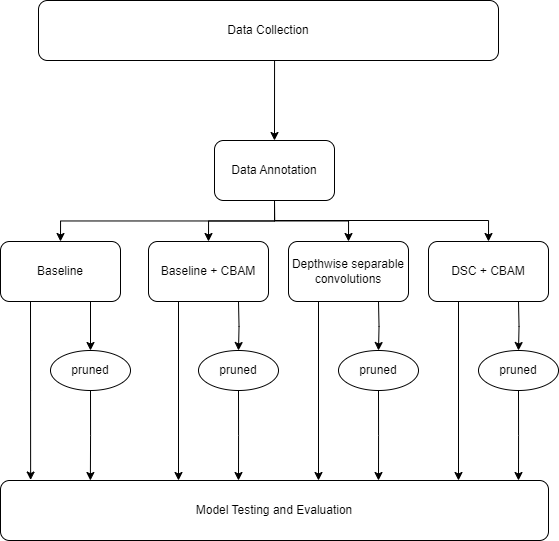
\includegraphics[width=0.92\linewidth]{images/DMIP-MethodologyFlowchart.png}}
    \caption{Methodology Flowchart}
    \label{fig:flowchart}
\end{figure}

The study aims to create a more efficient model capable of detecting masks in surveillance footage. Figure \ref{fig:flowchart} describes the process in the study, with the next sections further detailing the methods and pipeline.


\section{YOLOv3}

 YOLOv3 (You Only Look Once version 3) is a convolutional neural network (CNN) under the YOLO family capable of detecting objects and their respective class in a single evaluation. 

 The network is composed of a backbone network called Darknet-53, a neural network consisting of 53 convolutional layers that can extract numerous features from input images at multiple scales. Additionally, it utilizes a scale prediction method similar to a feature pyramid to detect objects in different scales \cite{redmonYOLOv3IncrementalImprovement2018}. This method alongside Darknet-53 allow YOLOv3 to detect objects and predict its categories at different scales and resolutions, resulting to the network being more accurate and robust to changes in object size and aspect ratio.

YOLOv3 uses several additional techniques such as multi-scale training and anchor boxes to further improve model performance. The multi-scale training technique allows the model to detect objects of different sizes by training it on images of various resolutions, whilst the anchor boxes are dimension clusters that predict the bounding boxes. A confidence score is added to the boxes to visualize the bounding box precision as well as the class prediction when an object is identified \cite{redmonYOLOv3IncrementalImprovement2018}. 

\section{Depthwise separable convolutions}

\begin{figure}[htbp]
    \centering
    \centerline{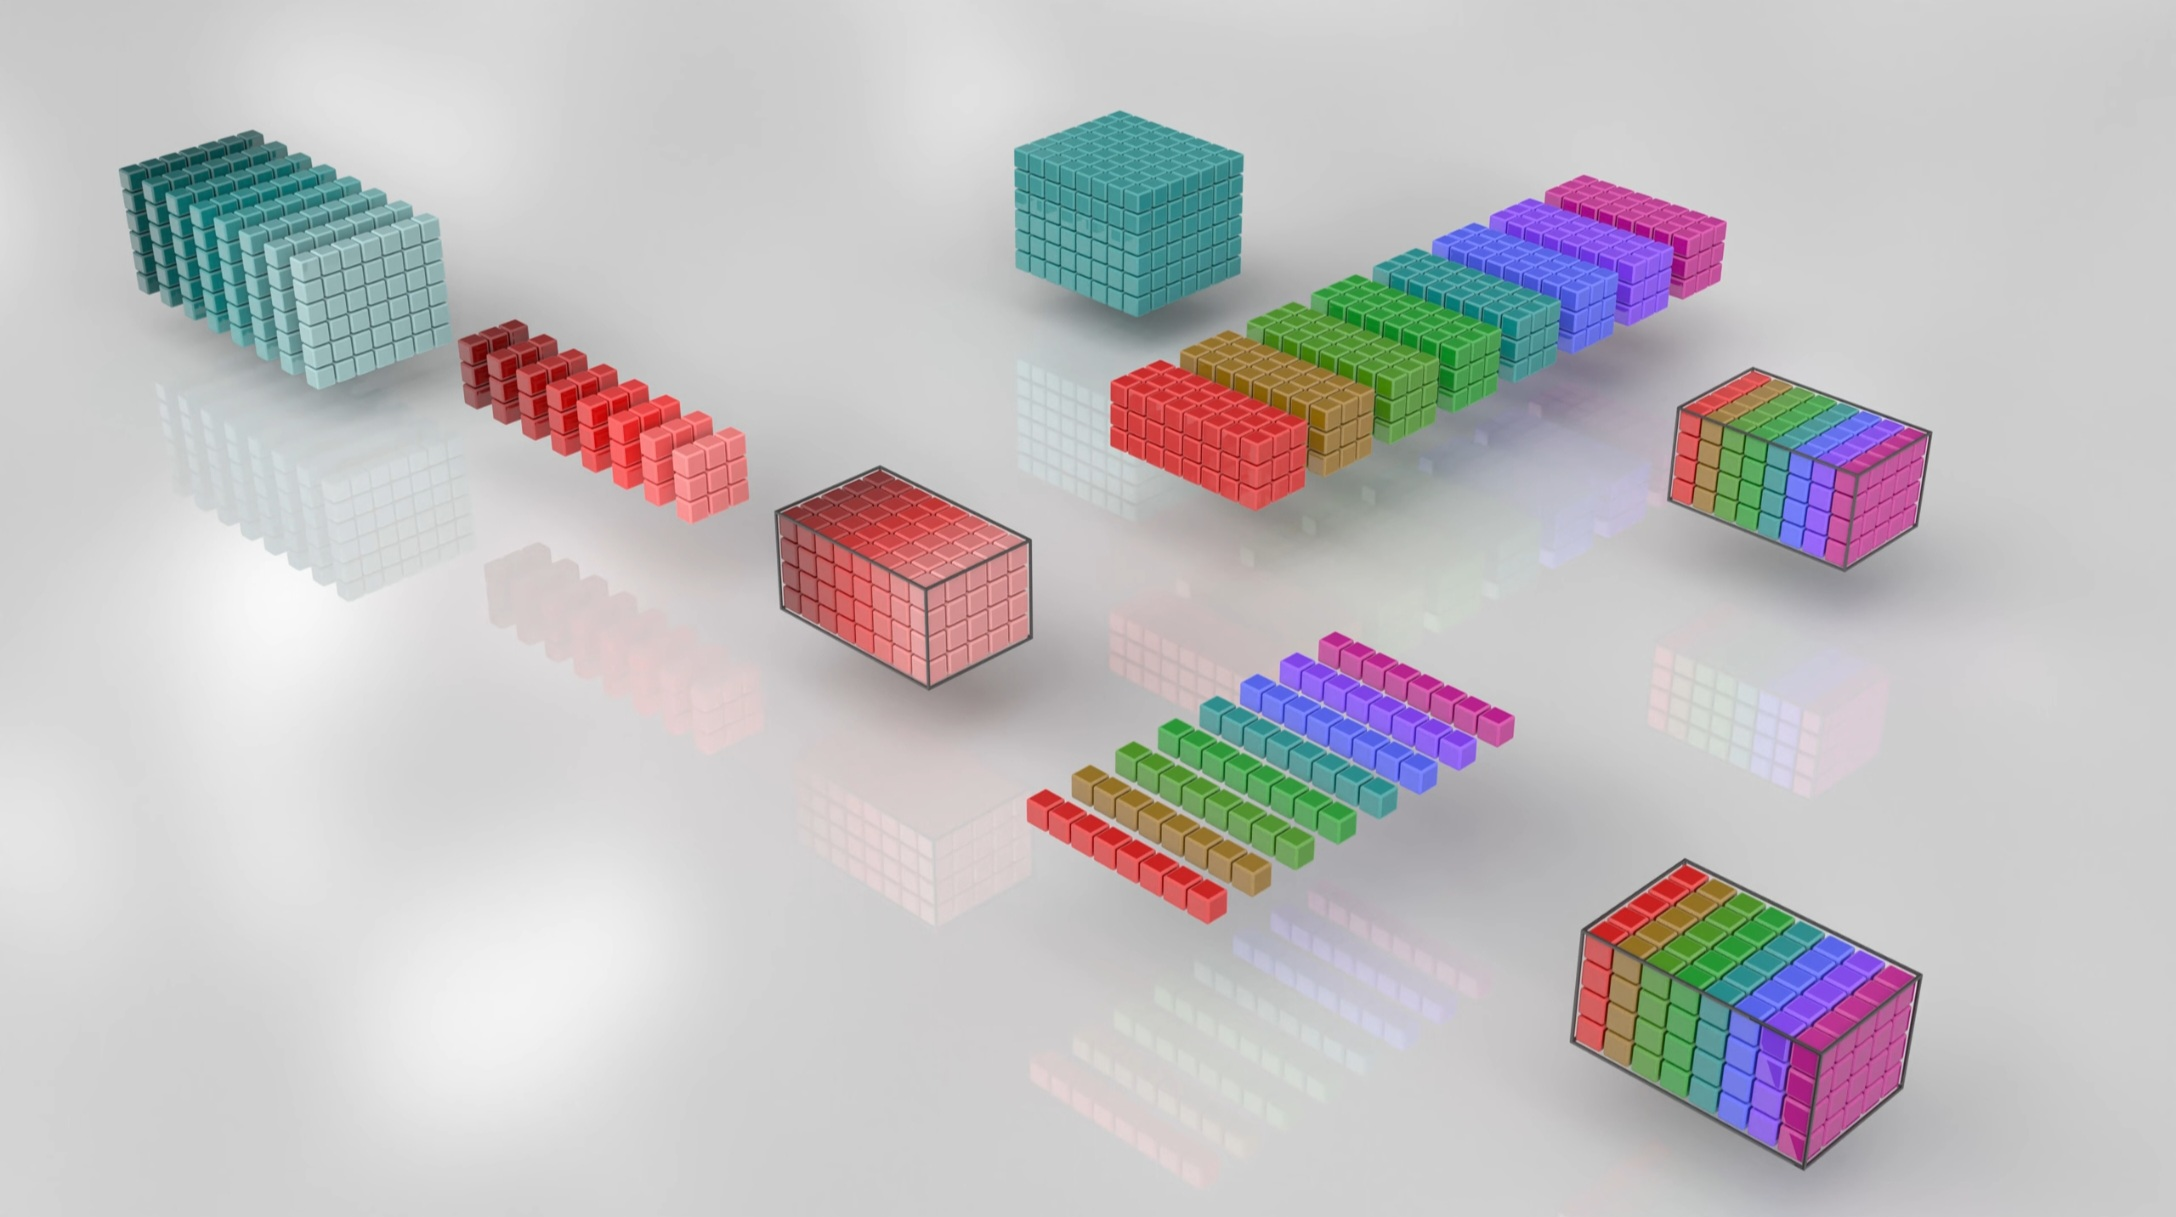
\includegraphics[width=0.8\linewidth]{images/DSC.jpg}}
    \caption{YOLO model for object detection \cite{animatedaiGroupsDepthwiseDepthwiseSeparable2023}}
    \label{fig:dsc_diagram}
\end{figure}

Figure \ref{fig:dsc_diagram} presents this comparison with depthwise separable convolutions on the left and with standard convolutional layers on the right. In a standard convolutional layer, the operation applies a 2D convolutional kernel with a size of \(K \times K\) across all input channels \(C_{in}\), resulting in a large number of parameters that need to be learned. The number of multiplications per output pixel for a standard convolution operation can be calculated as follows:
\[ Multiplications = K \times K \times C_{in} \times C_{out} \]
Depthwise separable convolutions on the other hand, splits this operation into two steps: a depthwise convolution and a pointwise convolution.

Depthwise convolution performs a spatial convolution independently on each input channel. It applies a separate filter of size \(K_d \times K_d\) that is smaller than the standard convolutional kernel to each input channel and produces an output feature map with the same number of channels as the input, which can be calculated as:
\[ Multiplications\_depthwise = K_d \times K_d \times C_{in}\]
The pointwise convolution then applies a 1x1 convolution to combine the outputs from the depthwise convolution (\(C_d\)) into the final output channels \(C_{out}\), which can be calculated as:
\[ Multiplications\_pointwise = 1 \times 1 \times C_d \times C_{out}\]
This step serves as a channel-wise linear combination and allows the network to learn complex interactions across the different channels \cite{cholletXceptionDeepLearning2017}.

Since the depthwise convolution applies a smaller number of filters to each channel independently, the number of multiplication computations required is significantly reduced as compared to a standard convolutional layer. Additionally, the pointwise convolution reduces the dimensionality of the feature maps, which further reduces the number of computations. The result, with the formula:
\[ Multiplications\_total = Multiplication\_depthwise + Multiplication\_pointwise\]
is a more computationally efficient and lightweight model that does not sacrifice too much accuracy and is better suited for deployment on devices with limited computational resources, as shown in table \ref{tab:dsccomparisons}.

\begin{table}[!htbp]
    \centering
    \caption{Model Parameter Count before and after applying depthwise separable convolutions}
    \resizebox{0.95\linewidth}{!}
    {
    \begin{tabular}{cccc}
          Model & Parameter Count & DSC Count & Reduction Percentage\\
          \hline
          baseline & 61,523,842 & 17,603,549 & 71.39\% \\
          \hline
          YOLO-BAM & 64,895,494 & 20,975,201 & 67.68\% \\
          \hline
    \end{tabular}
    }
    \label{tab:dsccomparisons}
\end{table}

However, it is important to note that depthwise separable convolutions have certain limitations or drawbacks. One such limitation is their sensitivity to input data. While these convolutions offer advantages in terms of reducing computational complexity and model size, they may struggle to capture complex spatial relationships and intricate patterns within the input data.

Due to their separable nature, depthwise separable convolutions apply separate filters to each input channel individually and then combine the results. This approach can limit the ability of the model to capture fine-grained spatial dependencies across different channels. In scenarios where the input data contains intricate spatial relationships or requires detailed feature extraction, depthwise separable convolutions may not perform as well as standard convolutions.

\section{Pruning}

\begin{figure}[htbp]
    \centering
    \centerline{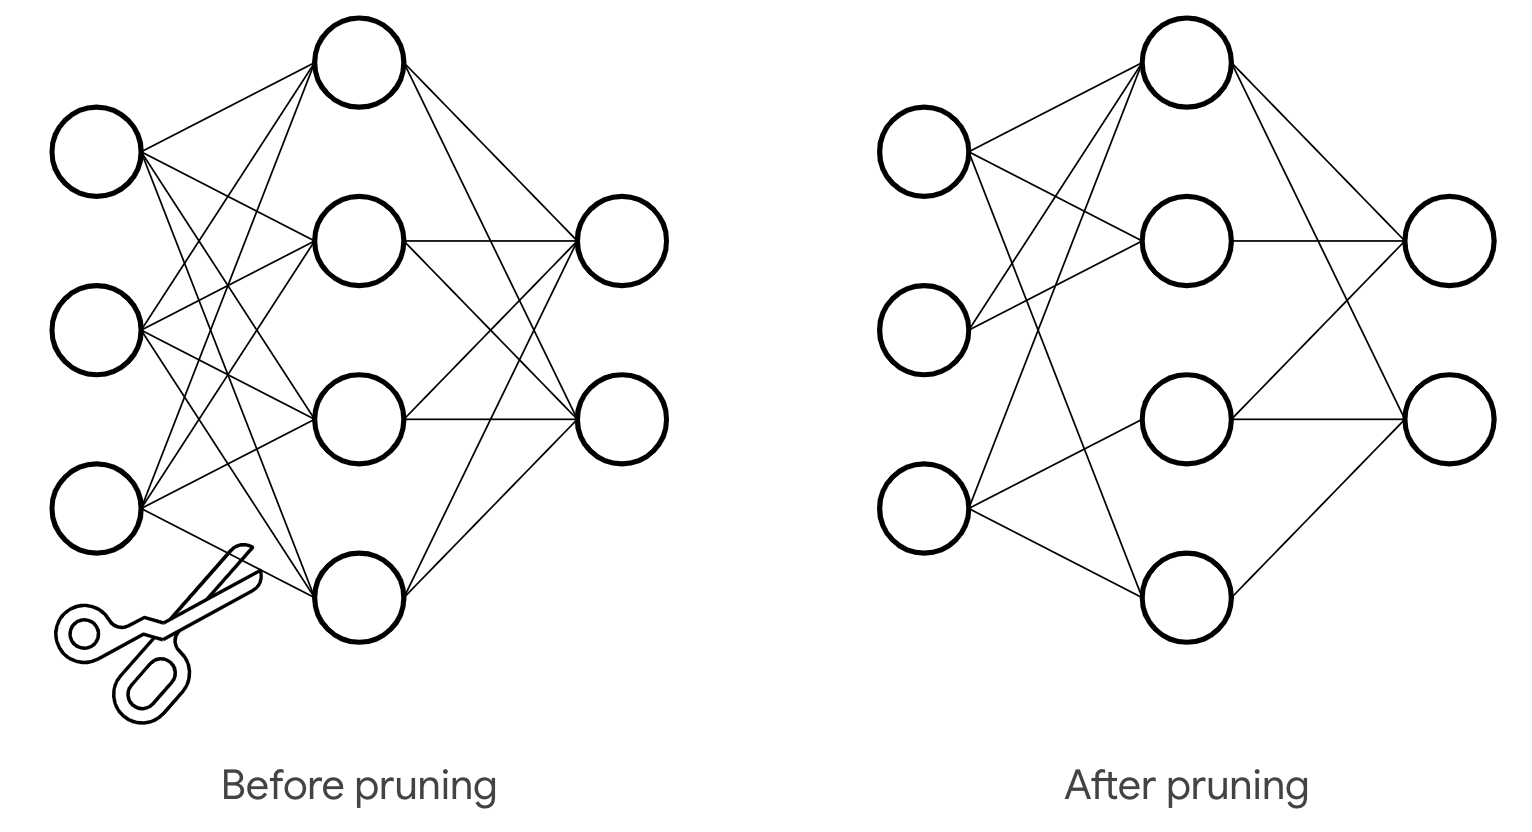
\includegraphics[width=0.8\linewidth]{images/pruning.png}}
    \caption{Pruning diagram \cite{TensorFlowModelOptimization}}
    \label{fig:pruning_diagram}
\end{figure}

Pruning is a neural network optimization technique that involves removing unnecessary parameters from a model to reduce its size, improve its computational efficiency, and potentially improve its performance in generalization. As shown in figure \ref{fig:pruning_diagram}, it involves identifying and removing the least important connections or neurons from the network and can be performed in different ways, including weight pruning, unit pruning, and filter pruning.

Filter pruning is a technique used to identify and remove the convolutional filters that contribute the least to a neural network's overall performance. The method identifies filters that produce low feature maps and remove them to reduce the overall size of the model. One particular study proposed a filter pruning technique that utilizes the L1-norm of the filters as a criterion for pruning. The method involves setting the weights of the filters to zero and then removing the filters with the smallest L1-norms. The pruning is done iteratively until the desired level of sparsity is achieved. The study showed that their pruning method can lead to significant compression of ConvNets without significant loss in accuracy \cite{liPruningFiltersEfficient2017}.

Pruning can be applied to various parts of the network, including the input layer, the hidden layers, and the output layer. In YOLOv3, for example, pruning can be applied to the detection "neck" and "head" parts of the network, which are responsible for feature extraction and object detection, respectively. The results of filter pruning to the models developed are shown in table \ref{tab:modelparaprunes}.

In the detection "neck" of YOLOv3, which consists of several convolutional layers, pruning can be applied to individual filters or channels to reduce the number of computations required for feature extraction. In the detection "head" part of YOLOv3, which consists of several fully connected layers, pruning can be applied to individual weights or neurons to reduce the size and complexity of the network.

\section{Attention blocks}
% REVISE THIS AS MUCH AS POSSIBLE TO REMOVE ANY SIGN OF CHATGPT ASSISTANCE

\begin{figure}[!htbp]
    \centering
    \centerline{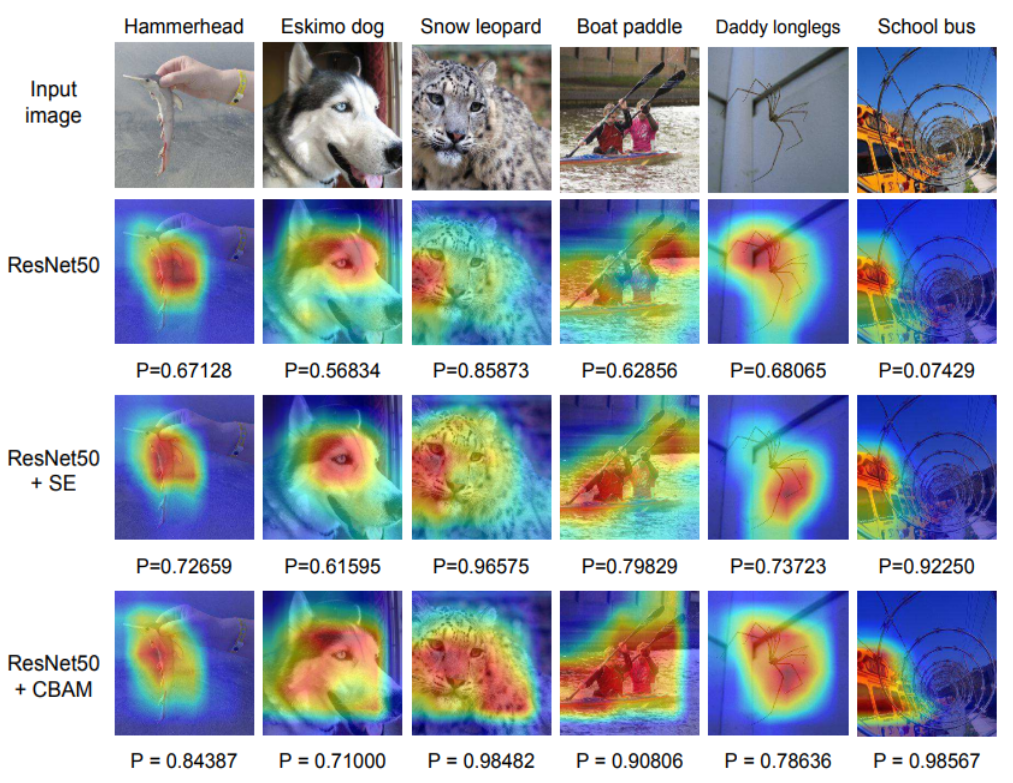
\includegraphics[width=0.8\linewidth]{images/attention.png}}
    \caption{Attention mechanism with highlighted areas \cite{wooCBAMConvolutionalBlock2018}}
    \label{fig:attention_diagram}
\end{figure}

Attention blocks are a component commonly used in deep neural networks to selectively focus on certain parts of the input data, allowing the model to prioritize important features and reduce noise in the input signal. Figure \ref{fig:attention_diagram} showcases this by displaying a Convolutional Block Attention Module which highlights most if not the entire object more accurately than other versions. Attention blocks have been used in a variety of different neural network architectures, including convolutional neural networks (CNNs), recurrent neural networks (RNNs), and transformer models, and have been shown to improve performance on a wide range of tasks, including image classification, machine translation, and speech recognition.

An attention block typically consists of three main components: a query matrix \(Q\), a key matrix \(K\), and a value matrix \(V\). These matrices, which are generated by applying different linear transformations to the input data, represent queries and keys of dimension \(d_k\), and values of dimension \(d_v\). The query matrix \(Q\) facilitates the computation of similarities between the input data and the elements in the key matrix \(K\). The similarity scores are subsequently utilized to determine the weights assigned to the corresponding values in the value matrix \(V\). The output matrix is then computed using the prescribed equation \cite{vaswaniAttentionAllYou2023}:
\[\text{Attention}(Q,K,V) = \text{softmax}(\frac{QK^T}{\sqrt{d_k}})V\]
The values are combined after weighting to produce an output that selectively focuses on the relevant parts of the input data.

In the context of YOLOv3, attention blocks can be implemented in the backbone network, which develops the feature maps. Specifically, attention blocks can be inserted in between convolutional layers to selectively attend to important parts of the feature maps. This can assist the network to better focus on object features and improve its detection performance.

Another way to implement attention blocks in YOLOv3 is to use them in the detection head, which predicts the bounding boxes, confidence scores, and class probabilities. Here, attention blocks can be used to weigh the extracted features from different scales of the feature pyramid, helping the network better localize objects at different scales.

The idea behind attention blocks is to create a set of learned weights that indicate how important each feature is to the output of the network. These weights can then be used to weight the features in a given layer, so that the model pays more attention to the most important features while ignoring those that are less important.

CBAM is integrated in all the convolutional layers except for the detection layers of the YOLO-BAM and DSCBAM models \cite{chakarDepthwiseSeparableConvolutions2020}.


\section{Pedestrian Detection Datasets}
\subsubsection{COCO}
The Common Objects in Context (COCO) dataset developed by the Microsoft research team is one of the largest image datasets suitable for the tasks of classification, segmentation, and captioning. The COCO 2017 dataset on Kaggle consists of over 118,000 trainable images which are labeled with multiple bounding boxes categorized into 80 classes such as 'bicycle' and 'car', as well as approximately 40,700 images for training. For the purposes of this study however, the YOLOv3 model was trained to classify images for the 'person' class.
\subsubsection{MOT}
\begin{figure}[!htbp]
\centering
\begin{subfigure}{.5\textwidth}
  \centering
  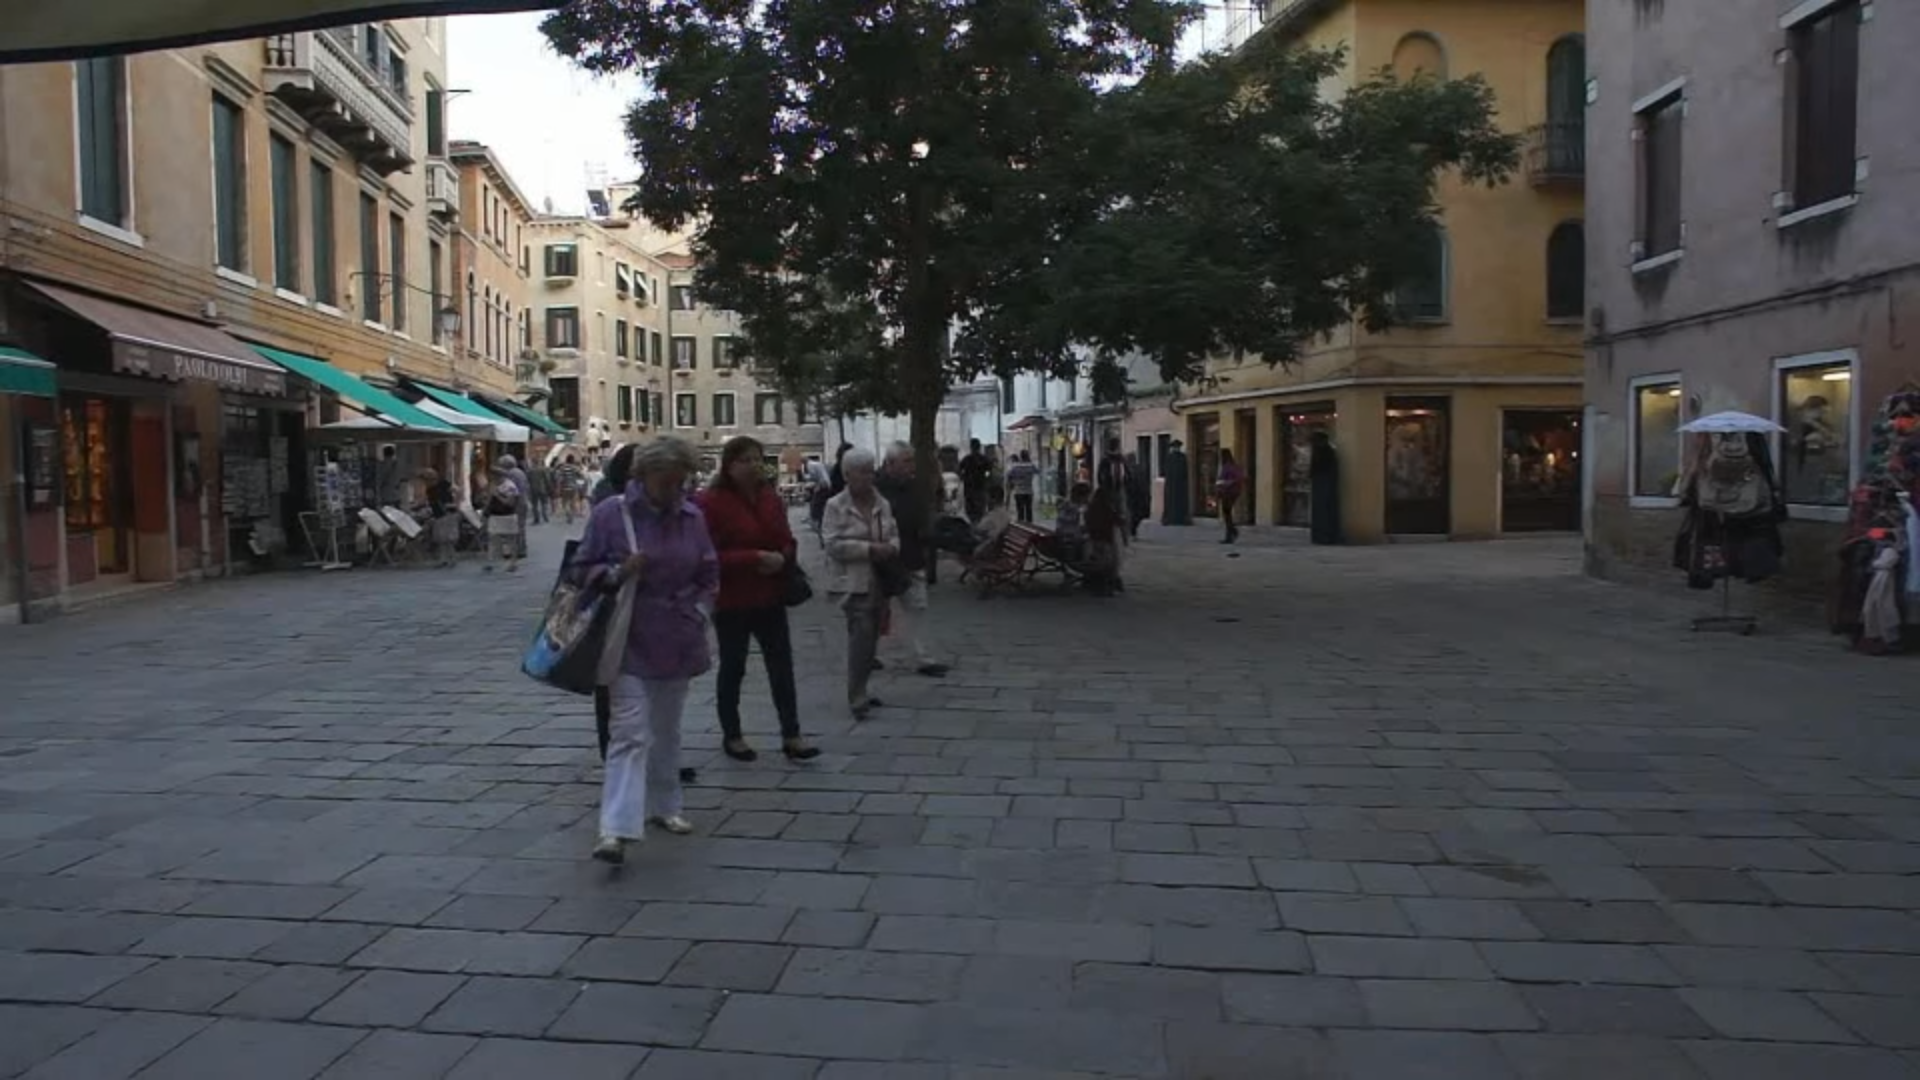
\includegraphics[width=0.9\linewidth]{images/MOT-02.png}
  \caption{A MOT17-02-SDP sequence frame}
  \label{fig:sub1}
\end{subfigure}%
\begin{subfigure}{.5\textwidth}
  \centering
  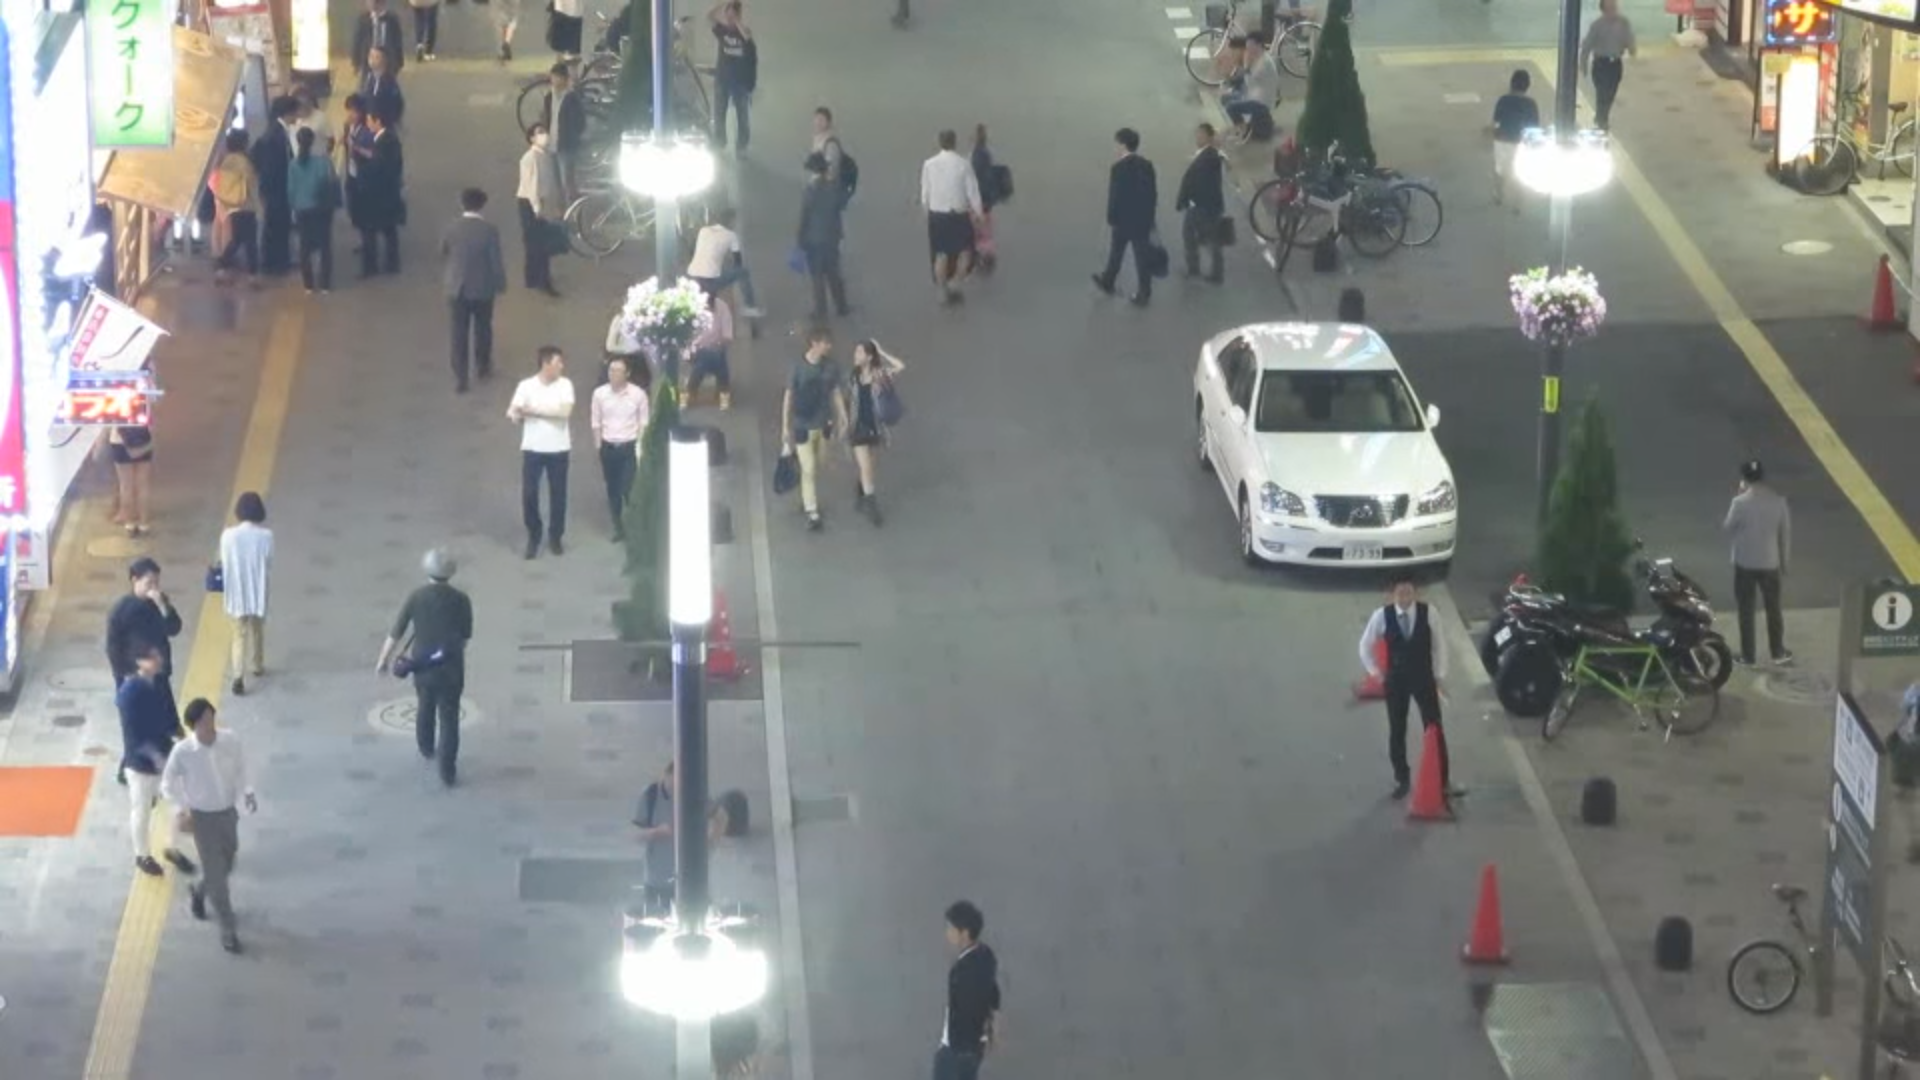
\includegraphics[width=0.9\linewidth]{images/MOT-04.png}
  \caption{A MOT17-04-SDP sequence frame}
  \label{fig:sub2}
\end{subfigure}
\caption{MOT17 Sequence showcase}
\label{fig:mot}
\end{figure}
The MOT17 (Multiple Object Tracking) dataset is a comprehensive benchmark in the field of computer vision and object tracking, offering a diverse collection of high-definition video sequences for multi-object tracking research. Comprising 14 distinct sequences with various challenges, such as occlusions, scale variations, and crowded scenarios, MOT17 provides ground truth annotations for tracking multiple objects over extended time frames. The study made use of two select sequences from the 2017 version of the dataset shown in figure \ref{fig:mot}, namely MOT17-02-SDP and MOT17-04-SDP whose camera positions remain static and reflect a normal and elevated viewpoint, respectively. The MOT17-02-SDP sequence contains 600 frames whereas the MOT17-04-SDP sequence contains 1050 frames.

\section{Software Implementation}
Training and testing of the YOLOv3 model and testing were conducted using the PyTorch library and the Python programming language. PyTorch is a free and open-sourced machine learning framework used for various machine learning applications such as image processing and natural language processing applications \cite{WhatPyTorch}.

\subsection{Hardware Implementation}
The models were trained on an Nvidia GTX 1070 GPU, with an Intel Core i7-8750H Processor and 16 GB of RAM.

\section{Metrics}
\subsection{Mean Average Precision (mAP)}
The mean average precision (mAP) serves as a vital metric for assessing the accuracy of detecting pedestrians in diverse scenarios. This metric measures the models' ability to accurately identify pedestrians amidst varying environmental conditions, such as different lighting, occlusions, and crowd densities. Higher mAP scores, using the formula
\[\text{mAP} = \frac{1}{C} \sum_{c=1}^{C} \text{AP}_c\]
indicate superior performance in accurately identifying pedestrians.

\subsection{Loss}
The loss function measures the disparity between the predicted output of the model and the ground truth labels for pedestrian detection. Lower loss values indicate improved performance in capturing the nuances of pedestrian appearances and spatial relationships in varying environments. The cross-entropy loss will be used in the study:
\[\text{Cross-Entropy Loss} = - \frac{1}{N} \sum_{i=1}^{N} \left( y_i \cdot \log(p_i) + (1 - y_i) \cdot \log(1 - p_i) \right)\]
where \(N\) is the number of samples in the dataset, \(y_i\) is the true label of the \(i\)-th sample, and \(p_i\) is the predicted probability of the \(i\)-th sample belonging to the positive class.

\section{Methodology Procedure}

\begin{figure}[!htbp]
    \centering
    \centerline{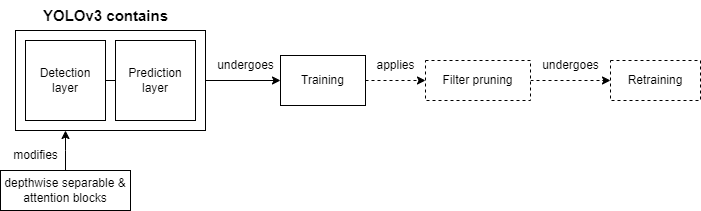
\includegraphics[width=0.95\linewidth]{images/Diagram.png}}
    \caption{Diagram of implementation}
    \label{fig:diagram}
\end{figure}

Figure \ref{fig:diagram} presents the flow to the implementation of the techniques utilized in the study. The broken line arrows and boxes signify additional techniques that may or may not be used by other model variants.

The baseline and every subsequent YOLOv3 implementation followed the Pytorch implementation of Aladdin Persson that is available on Github \cite{MachineLearningCollectionMLPytorch}. 

Each model variant replaced every convolutional layers except for the detection layers \cite{chakarDepthwiseSeparableConvolutions2020}. In addition to this, the modified convolution layers were fused with an attention block \cite{sunYoloBasedLightweightObject2023}. Using the COCO 2017 dataset, the models were trained for 50 epochs, with any additional notes taken regarding the respective models' runtime and metrics generated.

The models were first trained on the COCO dataset and then performed object detection on the MOT17-02-SDP and MOT17-04-SDP sequences, where the average FPS and inference time were recorded. The L1-norm scores for each filter in each layer of the trained model were computed and sorted. Once the L1-norm scores are sorted by value, around 30\% of the weights were pruned from the models. Pruning was done by zeroing the values of the weights. To compensate for this, the parameter count computed all the non-zeroed parameters. The models underwent retraining for the same number of epochs it takes for the baseline model to achieve a minimum 2\% difference in accuracy compared to its unpruned counterpart \cite{liPruningFiltersEfficient2017}. Further performance on the model was noted and compared for evaluation and analysis. 

\begin{table}[!htbp]
    \centering
    \caption{YOLO framework models}
    % \resizebox{0.70\linewidth}{!}
    {
    \begin{tabular}{cc}
        Model & Modifications \\ \hline 
        1& Baseline\\ 
        \hline 
        % 2& Baseline + filter pruning\\ 
        % \hline 
        2&Baseline + CBAM (YOLO-BAM)\\ 
        \hline 
        % 4&Baseline + CBAM + filter pruning\\
        % \hline
        3& Depthwise separable convolutions (DSC)\\
        \hline
        % 6& DSC + Filter pruning \\
        % \hline
        4& DSC + CBAM (DSCBAM)\\
        \hline
        % 8& DSC + CBAM + Filter pruning\\ \hline
    \end{tabular}
    }
    \label{tab:modelvars}
\end{table}

 Table \ref{tab:modelvars} presents the planned model variants and names, where the respective performance of each model such as accuracy and loss were listed down. The additional pruned model variants were also observed and compared to its unpruned versions.
 
In utilizing publicly available datasets for pedestrian detection, it is essential to emphasize that the models developed in this study were not designed to extract individual features for the purpose of identifying specific individuals. Instead, the focus was on modifying the YOLOv3 network for detecting pedestrians in surveillance scenarios. The study aimed to mitigate potential privacy risks by ensuring that any personally identifiable information that can indicate and identify specific individuals was removed during data collection. Additionally, the models were designed to prioritize the detection of generalized pedestrian shapes rather than individual features, further aligning with ethical considerations regarding privacy and personal identification.

\subsection{Statistical Analysis}
To enable a deeper understanding of the performance of the model variants, they will be evaluated with 10 sets of 10 test images for each category, totaling 400 unique images. Once the accuracies are generated, they will then be compared to the baseline YOLOv3 model using a paired two-tailed t-test, where the null and alternative hypotheses are:
\[H_{0} \text{ :  The models' performance is the same.}\] 
\[H_{\alpha} \text{ :  The models' performance is different.}\] 
The variants will be compared with each category to identify those that may be further investigated for future studies. The p-values generated from the t-test will be used to compare against the 95\% confidence interval (alpha = 0.05) to determine if the null hypothesis should be rejected.
